\documentclass[10pt]{beamer}
\usepackage[utf8]{inputenc}
\usepackage{hyperref}
\hypersetup{colorlinks=true,linkbordercolor=blue,linkcolor=white,urlcolor=blue,pdfborderstyle={/S/U/W 1}}

\usepackage[scaled]{helvet}
\usepackage[T1]{fontenc}
\usetheme{Berkeley}
\beamertemplatenavigationsymbolsempty
\setbeamertemplate{headline}{}
\setbeamersize{sidebar width left=1.5cm}
\setbeamerfont{section in sidebar}{size=\fontsize{6}{6}\selectfont}
\setbeamerfont{title in sidebar}{size=\fontsize{6}{6}\selectfont}
\title{Finding and removing duplicates}
\date{}

\begin{document}
\maketitle

\section{Topics}
\begin{frame}
\leftskip1em\textbf{Learn}
	\begin{itemize}
		\item to remove duplicates from the FoodChain-Lab database
	\end{itemize}
\vspace*{\fill}
Note: You need data from the tutorials \textcolor{blue}{\underline{\href{https://foodrisklabs.bfr.bund.de/data-collection-and-import/}{``Data collection and import''}}} and \textcolor{blue}{\underline{\href{https://foodrisklabs.bfr.bund.de/templatebacktracing/}{``Tracing backward template''}}}. Please do these tutorials first.
\end{frame}

\section{1}
\begin{frame}
	\begin{center}
			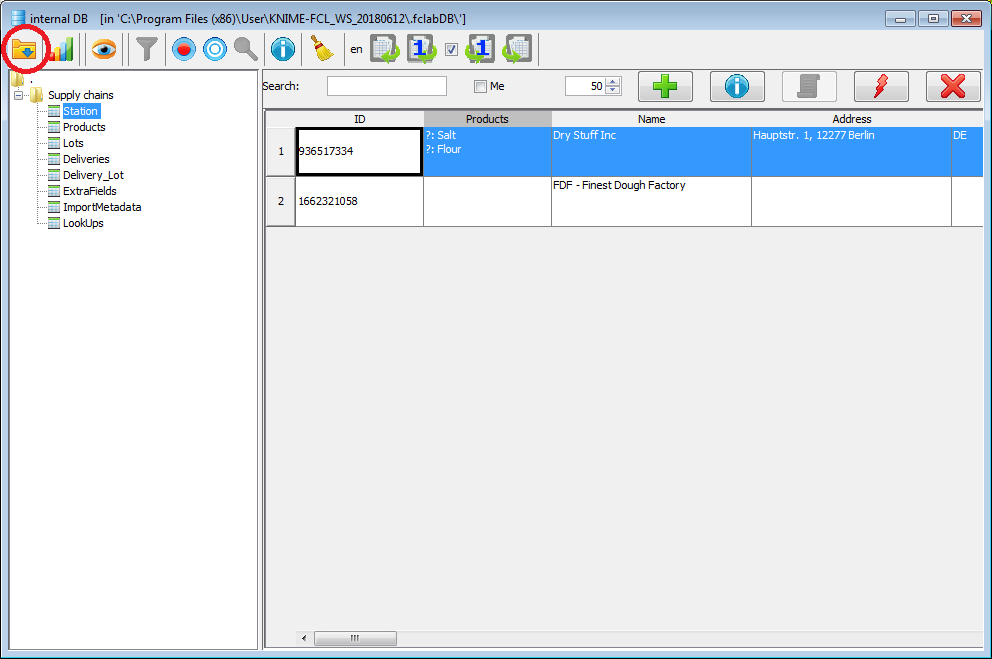
\includegraphics[height=0.6\textheight]{1.png}
	\end{center}
	\begin{itemize}
		\item Open the database and import \textcolor{blue}{\underline{\href{https://github.com/SiLeBAT/BfROpenLabResources/raw/master/GitHubPages/documents/FCL\_Finding\_And\_Removing\_Duplicates/FCL\_Backtrace\_Start\_tob\_en\_FDF\_DB\_clean.xlsx}{``FCL\_Backtrace\_Start\_tob\_en\_FDF\_DB\_clean.xlsx''}}}.
		\item Start the similarity search (see button in the red circle).
	\end{itemize}
\end{frame}

\section{2}
\begin{frame}
	\begin{center}
			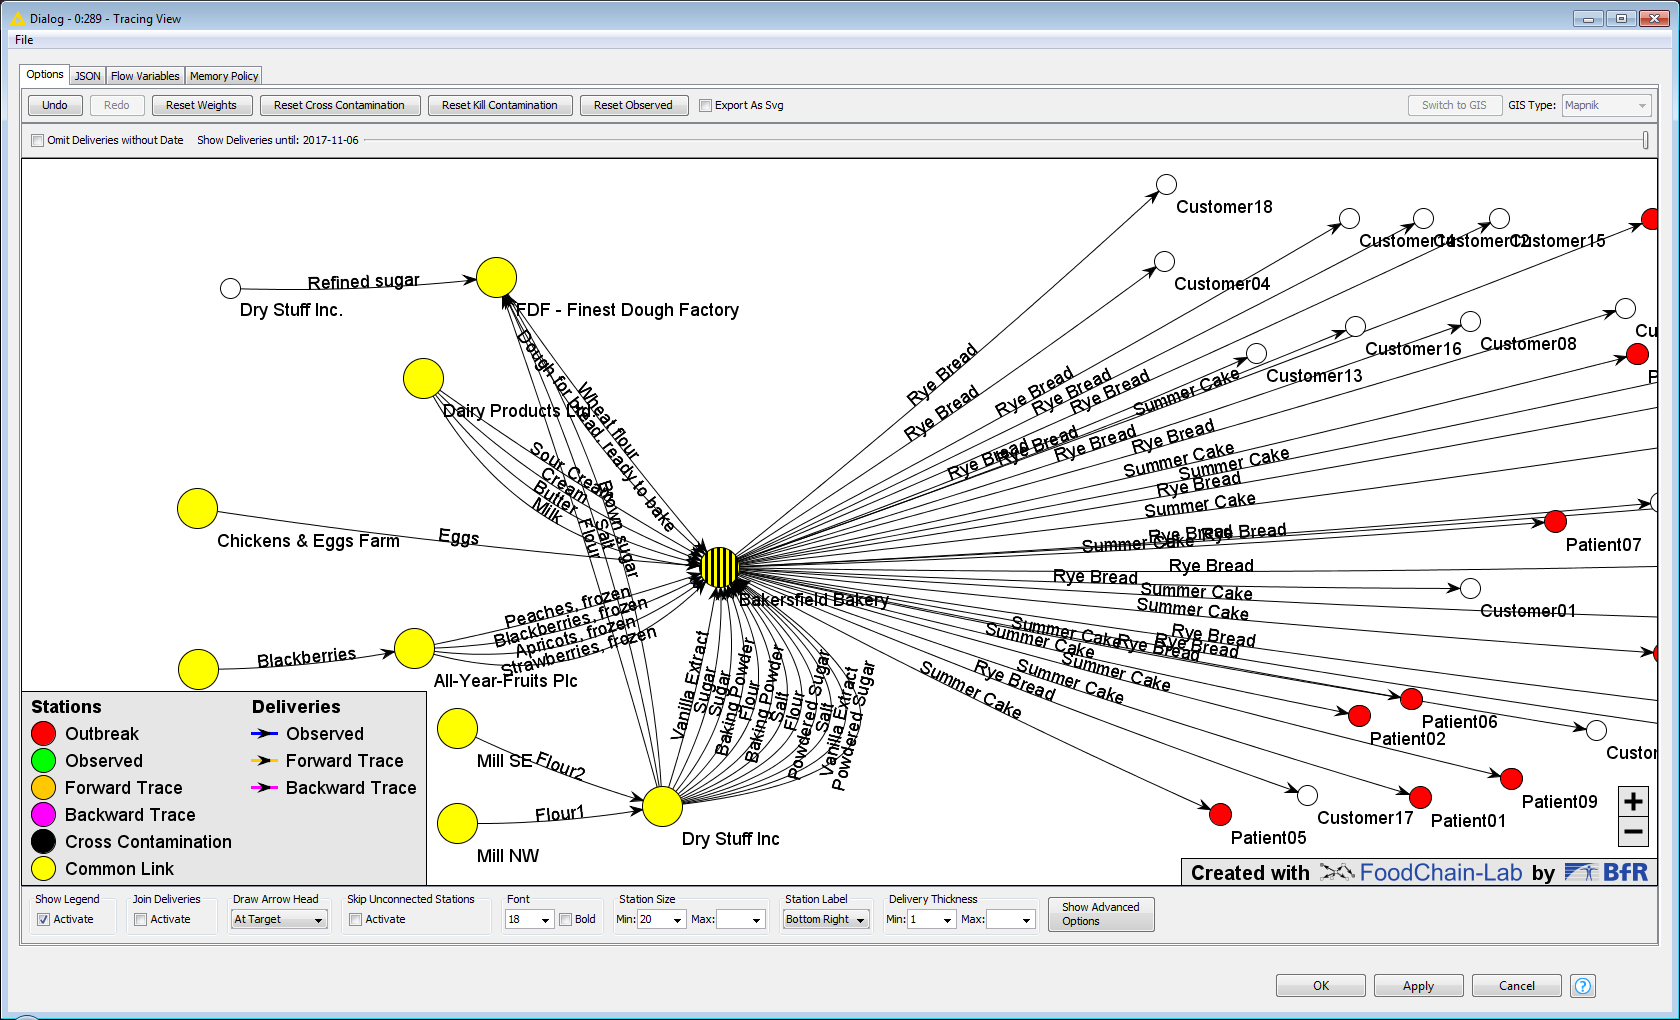
\includegraphics[scale=0.4]{2.png}
	\end{center}
	\begin{itemize}
		\item To search for duplicates in station names and addresses tick the encircled radio button.
		\item ``Name: 90'' means that the similarity between two or more station names must be 90 \% or greater in order to be displayed as duplicate.
		\item Click ``OK''
	\end{itemize}
\end{frame}

\section{2}
\begin{frame}
	\begin{center}
			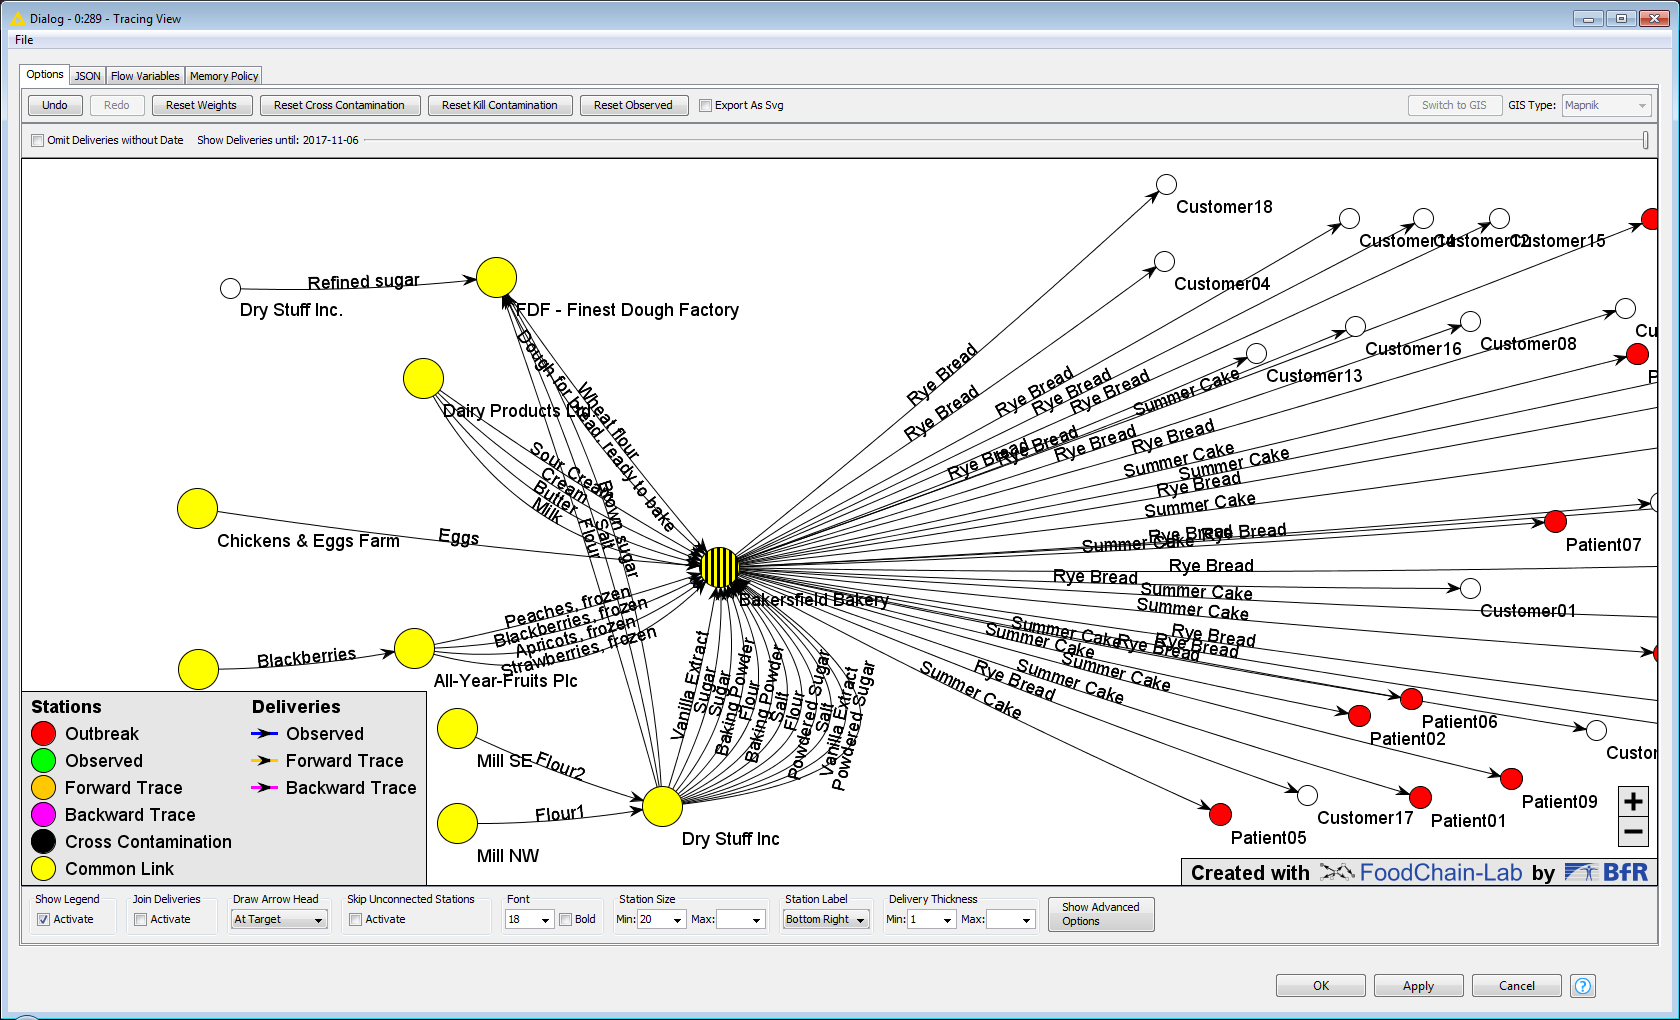
\includegraphics[scale=0.4]{2.png}
			%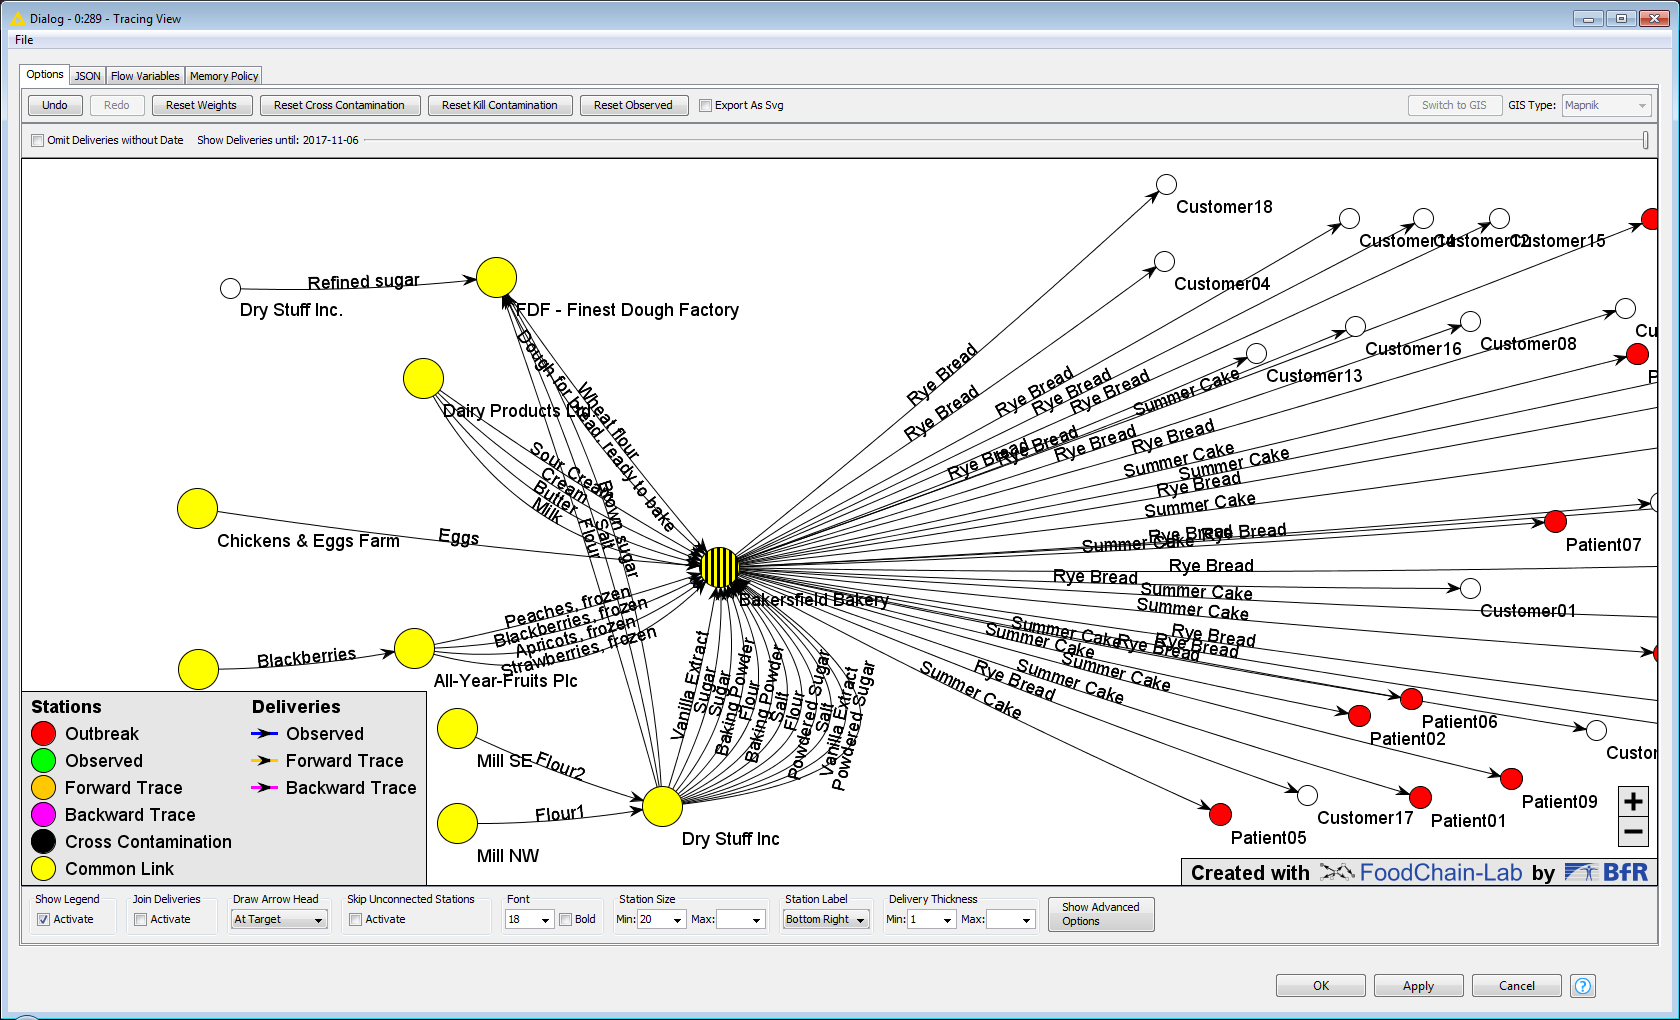
\includegraphics[width=0.9\columnwidth]{2.png}
	\end{center}
	\begin{itemize}
		\item To search for duplicates in station names and addresses tick the encircled radio button.
		\item ``Name: 90'' means that the similarity between two or more station names must be 90 \% or greater in order to be displayed as duplicate.
		\item Click ``OK''
	\end{itemize}
\end{frame}

Left click and hold the duplicate row and drop it onto the row that should be kept. It is like moving a file (or a selection of files) to a folder in a file browser. In this case

\end{document}
